\chapter{General framework of \smtrat}
\label{chapter:generalframework}


Our toolbox has a modular \Cpp class design which can be used to
compose NRA theory solvers for an SMT embedding in a \emph{dynamic}
and \emph{hierarchic} fashion. Our NRA theory solvers are instances of
\managerClass, which offers an interface to communicate with the
environment and which coordinates the satisfiability check according
to a user-defined \strategyClass. Such a strategy combines basic NRA
theory solver modules, derived from \moduleClass. 
%NRA theory problems are specified using the \formulaClass class. Basic
%NRA theory solver modules are derived from the \moduleClass class.
%Such modules can be embedded into a \managerClass, which offers an
%interface to communicate with the environment and which coordinates
%the satisfiability check according to a user-defined 
%\strategyClass.
Figure~\ref{fig:framework} shows an example configuration. Moreover, a
\Java-based graphical user interface (GUI) can be used for an
intuitive and user-friendly specification of strategies (and the
automatic generation of a corresponding \strategyClass class). Next,
we briefly describe these concepts. 

\smtrat is a \Cpp library consisting of a collection of
SMT-compliant modules which can be combined to (1) a 
theory solver in order to extend the supported logics of an
existing SMT solver by non-linear real arithmetic and (2) to
SMT solver in which these modules can be (and most of them are) 
integrated to tackle RCF. The
latter is intended to be a testing environment for the development of
SMT-compliant theory solvers, as the one presented in this paper.
\smtrat defines three types of components (see Appendix 
\ref{app:smtrat}): \emph{manager}, \emph{strategy} and \emph{module}. 
% In addition, a frontend (1) provides the interfaces to an extern SMT 
%solver or (2) parses the input file to an RCF formula.
In the following we first describe the functionality of a module and
show how the manager composes different modules according to a
strategy to a solver.

\section{The \formulaClass class} \formulaClass instances contain,
besides a sequence of NRA constraints, a bitvector storing some
information about the problem and the history of its check. E.g.,
there is a bit which is $1$ if some of the constraints are equations.
Also for each module there is a bit which is $1$ if the module was
already invoked on the given problem. Such information can be used to
specify conditions under which a procedure should be invoked for a
certain problem.\smallskip

\section{The \moduleClass class} A module $m$ contains a set of
formulas, called its \emph{set of received formulas}, we denote by 
$\Crcv(m)$. The main
procedure of a module is \texttt{isConsistent()} and either decides
whether $\Crcv$ is satisfiable or not returning \SAT or \UNSAT,
respectively, or returns \UNKNOWN. Note, that a set of formulas is
semantically defined by their conjunction. We can manipulate the set
of received formulas by adding (removing) formulas $\varphi$ to (from)
it with \texttt{add($\varphi$)} (\texttt{remove($\varphi$)}). Since in
the SMT embedding $\Crcv$ is usually changed between two consecutive
\texttt{isConsistent()} calls only by adding/removing constraints, the
solver's performance can be significantly improved if the modules can
make use of the results of previous checks, that is they support
\emph{incrementality} and \emph{backtracking}. In case that the module
determines the unsatisfiability of $\Crcv$, it is expected to compute
at least one preferably small \emph{infeasible subset} $\Cinf\subseteq
\Crcv$. Moreover, a module has the possibility to name lemmas, which
are formulas being tautologies, that is they hold for all assignments
of the variables occuring in them. These lemmas should encapsulate
information which can be extracted from a module's internal state and
propagated among other \smtrat modules. Furthermore, \smtrat provides
the feature that a module itself can ask other modules for the
satisfiability of the set $\Cpass$ of formulas, called its \emph{set
of passed formulas}, using the procedure \texttt{runBackends()} which
is controlled by the manager. 

\begin{figure}[t]
\caption{A snapshot of an \smtrat composition embedded in an SMT solver.}
\begin{center}
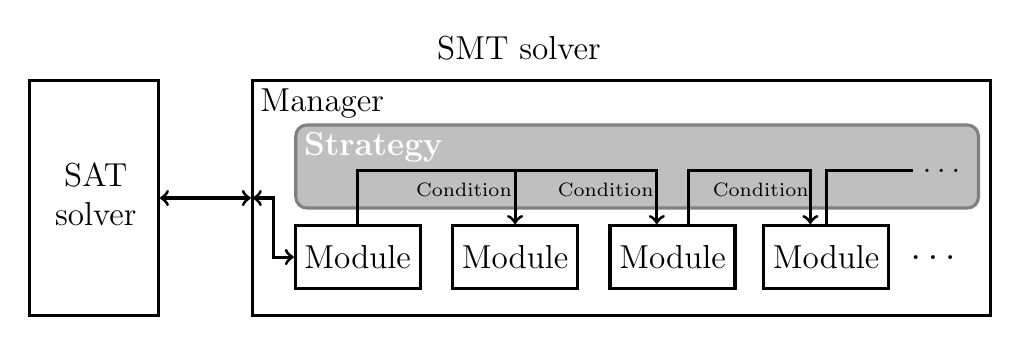
\begin{tikzpicture}[every node/.style={rectangle}, text centered, bend angle=15, scale=1, line width=.4mm]
	\node[] (smtsolver) at (-2.5, 2.2) {\large SMT solver};
	\node[draw, minimum height=85pt, text width=40pt] (satsolver) at (-7.9, 0.3) {\large\begin{tabular}{c}SAT \\ solver\end{tabular}};
	\node[draw, minimum height=85pt, text width=260pt] (manager) at (-1.2, 0.3) {};
	\node[] (managerText) at (-5, 1.5) {\large Manager};
	\node[fill=lightgray,draw=gray, rounded corners, minimum height=30pt, text width=240pt] (strategy) at (-1,.7) {};
	\node[] (strategyText) at (-4.35, .95) {\large\bf \color{white} Strategy};
	\draw[<->] (-5.36,-.45) -- (-5.62,-.45) -- (-5.62,.3) -- (-5.88,.3);
	\draw[->] (-4.55,-.03) -- (-4.55,.65) -- (-.75,.65) -- (-.75,-.03);
	\node[] (strategyText) at (-1.4, .4) {\scriptsize Condition};
	\draw[->] (-2.55,.65) -- (-2.55,-.03);
	\node[] (strategyText) at (-3.2, .4) {\scriptsize Condition};
	\draw[->] (-.35,-.03) -- (-0.35,.65) -- (1.2,.65) -- (1.2,-.03);
	\node[] (strategyText) at (.57, .4) {\scriptsize Condition};
	\draw (1.4,-.03) -- (1.4,.65) -- (2.5,.65);
	\node[] (dotsa) at (2.9,.65) {\large \ldots};
	\node[draw, minimum height=23pt] (moduleAText) at (-4.55, -.45) {\large Module};
	\node[draw, minimum height=23pt] (moduleBText) at (-2.55, -.45) {\large Module};
	\node[draw, minimum height=23pt] (moduleCText) at (-.55, -.45) {\large Module};
	\node[draw, minimum height=23pt] (moduleDText) at (1.4, -.45) {\large Module};
	\node[] (dotsc) at (2.8, -.45) {\Large \ldots};
	\path[<->] (satsolver.0) edge[] node[left] {} (manager.180);
\end{tikzpicture}

\end{center}
\label{fig:framework}
\end{figure}

\section{The \managerClass and the \strategyClass class} A
\emph{strategy} is a directed tree $T:=(V, E)$ with a set $V$ of
module instances as nodes and $E\subseteq V\times \Omega\times V$,
where $\Omega$ is a set of conditions. The \emph{manager} contains the
strategy and the input formula $C_{input}$, either received by a prefexed solver
or parsed from an example file. Furthermore, it maintains the
allocation of module instances as follows. Initially, the manager calls the method
\texttt{isConsistent()} of the module instance given by the root of
the strategy with $\Crcv = C_{input}$ being the set of received formulas of this
module. Whenever a module instance $m\in V$ calls
\texttt{runBackends()}, with $\Cpass$ being its set of passed
formulas, the manager calls \texttt{isConsistent()} of each module instance
$m'$ with \Crcv' = \Cpass being its set of received formulas, for which
an edge $(m, \omega, m')\in E$ exists such that $\omega$ holds for
$\Cpass$, and passes the results back to $m$. Furthermore, it also
passes back the infeasible subsets and lemmas provided by the invoked
modules. The module $m$ can now benefit in its solving and reasoning
process from this shared information.
%In the following we write short $(m, m')$ for $(m, \omega, m)$ if 
%$\omega = \True$.

